

\documentclass[a4paper,11pt]{article}
\usepackage{amsmath,amssymb,amsfonts,amsthm, mathrsfs}
\usepackage{tikz}
\usepackage [utf8x] {inputenc}
\usepackage [T2A] {fontenc} 
\usepackage[russian]{babel}
\usepackage{cmap} 
\RequirePackage{caption}
\DeclareCaptionLabelSeparator{defffis}{. }
\captionsetup{justification=centering,labelsep=defffis}

\usepackage[mathscr]{eucal}
\usepackage{braket}
% Так ссылки в PDF будут активны
\usepackage[unicode]{hyperref}
\usepackage{mathtools}


% вы сможете вставлять картинки командой \includegraphics[width=0.7\textwidth]{ИМЯ ФАЙЛА}
% получается подключать, как минимум, файлы .pdf, .jpg, .png.
\usepackage{graphicx}
% Если вы хотите явно указать поля:
\usepackage[margin=1in]{geometry}
% Или если вы хотите задать поля менее явно (чем больше DIV, тем больше места под текст):
% \usepackage[DIV=10]{typearea}

\usepackage{fancyhdr}

\newcommand{\bbR}{\mathbb R}%теперь вместо длинной команды \mathbb R (множество вещественных чисел) можно писать короткую запись \bbR. Вместо \bbR вы можете вписать любую строчку букв, которая начинается с '\'.
\newcommand{\eps}{\varepsilon}
\newcommand{\bbN}{\mathbb N}
\newcommand{\dif}{\mathrm{d}}
%\usepackage[cal=boondox]{mathalfa} %todo

\pagestyle{fancy}
\makeatletter % сделать "@" "буквой", а не "спецсимволом" - можно использовать "служебные" команды, содержащие @ в названии
\fancyhead[L]{\footnotesize}%Это будет написано вверху страницы слева
\fancyhead[R]{\footnotesize Karamyshev Anton}
%\fancyfoot[L]{\footnotesize \@author}%имя автора будет написано внизу страницы слева
\fancyfoot[R]{\thepage}%номер страницы —- внизу справа
\fancyfoot[C]{}%по центру внизу страницы пусто.
\renewcommand{\maketitle}{%
	\noindent{\bfseries\scshape\large\@title\ \mdseries\upshape}\par
	\noindent {\large\itshape\@author}
	\vskip 2ex}
\makeatother
\def\dd#1#2{\frac{\partial#1}{\partial#2}}

\usepackage{xcolor}


\bibliographystyle{acm}% Choose Phys. Rev. style for bibliography

\author{Karamyshev}

\begin{document}

Рассматривается четырехкубитный квантовый протокол распределения ключей, базирующийся на измерении пар состояния Белла. Кубиты объединяются в единый блок, передаваемый от отправителя к получателю в каждом сообщении. Шифрование здесь осуществляется путем случайной группировки четырех отдельных кубитов в две новые пары, аналогичный механизм также является одним из способов обнаружить подслушивающее устройство в квантовом канале. Незамедлительно после приёма блока кубитов приемник случайным образом разбивает четыре кубита на пары и проверяет их при помощи измерений состояний Белла. Из сравнения информации о группировке этих четырех кубитов обе стороны соединения могут обнаружить нелегального пользователя в канале. В предложенном протоколе приемник обрабатывает блок мгновенно во время получения, что является эффективным способом преодоления ультракороткого времени хранения квантового состояния.



\section{История и предпосылки}

Квантовое распределение ключей (англ.: Quantum Key Distribution, QKD) — метод передачи ключа, который использует квантовые явления для гарантии безопасной связи. Этот метод позволяет двум сторонам, соединенным по открытому каналу связи, создать общий случайный ключ, который известен только им, и использовать его для шифрования и расшифрования сообщений.


В настоящее время предложено довольно много работ по данной тематике. Самый первый протокол QKD был предложен Беннеттом и Брассардом в 1984 году. Данный протокол получил название BB84 и базировался на использовании двух взаимно несмещенных состояний поляризации фотонов \cite{BB84}. Авторами был описан способ распределения случайного секретного ключа между Алисой и Бобом. 
 
Позднее Экерт предложил другой протокол QKD \cite{E91}, названный E91, основанный на парадоксе Эйнштейна-Подольского-Розена \cite{EPR}. После этого были теоретически предложены и экспериментально реализованы различные протоколы QKD, например, базирующиеся на однофотонных \cite{liang2015simple} и множественных состояниях \cite{fourstate}. Среди этих работ для переноса информации широко используются фотоны, поскольку ими легко манипулировать и они передают информацию со скоростью света.

Новый виток в развитии QKD связан с использованием состояний Белла \cite{EPR}.
В качестве квантового канала состояние Белла было впервые предложено в \cite{Gao} и подтверждено \cite{bellstatescomp} как максимально запутанное состояние двухкубитной квантовой системы. Кроме того, по сравнению с другими мультикубитными состояниями (состояния W \cite{W}, GHZ \cite{GHZ} и кластерные состояния \cite{cluster}), состояние Белла легче всего реализовать с помощью нелинейного процесса, описанного в  \cite{twophotons}. 

В основополагающей работе \cite{Gao} две стороны разделяют секретный ключ, сравнивая форму начального состояния Белла и результат измерения состояния Белла после квантовой перекрутки %todo.
Затем \cite{nine} повысил общую эффективность коммуникации до 100\% по сравнению с достигнутыми 50\% в \cite{Gao}. В \cite{ten} представлен первый аутентифицированный полуквантовый протокол распределения ключей без использования аутентифицированных классических каналов, основанный на состояниях Белла.

Авторы \cite{Gao} и \cite{nine} предложили два протокола QKD, которые используют состояния Белла, распределенные между отправителем и получателем, которых в дальнейшем будет называть Алисой и Бобом соответственно. В их протоколах две пары состояний Bell разделены между двумя сертифицированными сторонами связи. Отправитель и получатель хранят по два кубита, запутанные друг с другом. После одновременного измерения состояния Белла (BSM) с двух сторон реализуется квантовая запутанность уже между четырьмя кубитами.

В недавней работе \cite{base} было предложено усовершенствование \cite{ten} для предотвращения подслушивания с более низким коэффициентом ошибок при подтверждении сообщений, а также с более быстрым обнаружением битов ключа, основанных на четырехкубитном состоянии, которое состоит из двух пар состояний Белла. Дальнейшая речь пойдёт о протоколе, представленном в \cite{base}.

\section{Протокол QKD на основе случайных группировок и измерений состояний Белла}

\subsection{Основные идеи}
Рассматриваемый протокол предполагает использование четырёхкубитных конфигураций, состоящих из двух пар состояний Белла. Каждый раз передатчик (Алиса) подготавливает группу, состоящую из четырёх кубитов, для незамедлительной отправки приёмнику (Бобу). Боб производит измерение квантового состояния сразу же после получения всей партии кубитов. Это односторонний процесс, что является важным нововведением по сравнению с двусторонними протоколами, в которых квантовое состояние должно сохраняться до завершения передачи \cite{Gao,nine}, благодаря которому протокол может преодолеть проблему ультракороткого времени когерентности квантовых состояний.

Если приводить более формальное описание, то можно обозначить четыре кубита двух состояний Белла как $P_1$, $P_2$, $P_3$ и $P_4$. Условимся, что квантовая запутанность имеет место между $P_1$ и $P_2$, а также между $P_3$ и $P_4$. После измерения состояний Белла с обеих сторон запутанными оказываются $P_1$ и $P_3$, $P_2$ и $P_4$ соответственно. Базисные функции состояний Белла выражаются следующим образом:
\begin{equation*}
\ket{\phi^{\pm}} = \dfrac{1}{\sqrt2}\big(\ket{00} \pm \ket{11} \big), \quad
\ket{\psi^{\pm}} = \dfrac{1}{\sqrt2}\big(\ket{01} \pm \ket{10} \big).
\end{equation*}


\iffalse ... 
\begin{table}
	\centering
	\caption{\label{tab:1}Соответствие состояний Белла и бинарной случайной последовательности.}
	\begin{tabular}{ |c||c||c| }
		\hline
		$(P_1, P_3)$ & $(P_1, P_3)$ & $\mathcal{K}$ \\ \hline
		$\ket{\phi^+}$ & $\ket{\phi^-}$ & 00 \\ 
		$\ket{\phi^-}$ & $\ket{\phi^+}$ & 01 \\ 
		$\ket{\psi^+}$ & $\ket{\psi^-}$ & 10 \\ 
		$\ket{\psi^-}$ & $\ket{\psi^+}$ & 11 \\ 
		\hline
	\end{tabular}
\end{table}

\begin{table}
	\centering
	\caption{\label{tab:2}Различные группировки кубитов для Боба.}
	\begin{tabular}{ |c||c||c| }
		\hline
		Bob's grouping & Verdict & Announced number \\ \hline
		$(P_1, P_3)\&(P_2, P_4)$ & Right & 1 \\
		$(P_1, P_2)\&(P_3, P_4)$ & Wrong & 0 \\
		$(P_1, P_4)\&(P_2, P_3)$ & Wrong & 0 \\
		\hline
	\end{tabular}
	
\end{table}

\fi

Например, если начальными состояниями Белла были $\ket{\phi^-}$ и $\ket{\phi^+}$, то общее запутанное состояние из четырёх кубитов запишется следующим образом:

\begin{align}\label{state}
\ket{\mathcal{C}}_{1234} &= \ket{\phi^-}_{12} \otimes \ket{\phi^+}_{34} = \nonumber \\
&= \dfrac{1}{2} \Big(\ket{\phi^+}_{13} \ket{\phi^-}_{24} + 
 					\ket{\phi^-}_{13} \ket{\phi^+}_{24} +
 					\ket{\psi^+}_{13} \ket{\psi^-}_{24} +
 					\ket{\psi^-}_{13} \ket{\psi^+}_{24} \Big),
\end{align}

где индексы $1$, $2$, $3$ и $4$ обозначают номер связанного кубита, а $\otimes$ обозначает операцию тензорного произведения.


Из \eqref{state} видно, что состояние становится суперпозицией четырех состояний, это означает, что мы можем получить четыре различных результата при измерении комбинаций состояний Белла. Также обратим внимание, что уравнение \eqref{state} представляет лишь одну из возможных комбинаций, подробный анализ всех состояний можно найти в \cite{base,entang}. Вкратце, существует несколько форм случайной группировки этих четырех кубитов, из которых только одна группировка определена как правильная. Это основной метод шифрования информации во время коммуникации. Предлагаемый протокол показан на рис.~\ref{im1}, где Алиса и Боб являются сертифицированными отправителем и приемником соответственно.

\begin{figure}[h!]
	\centering    
	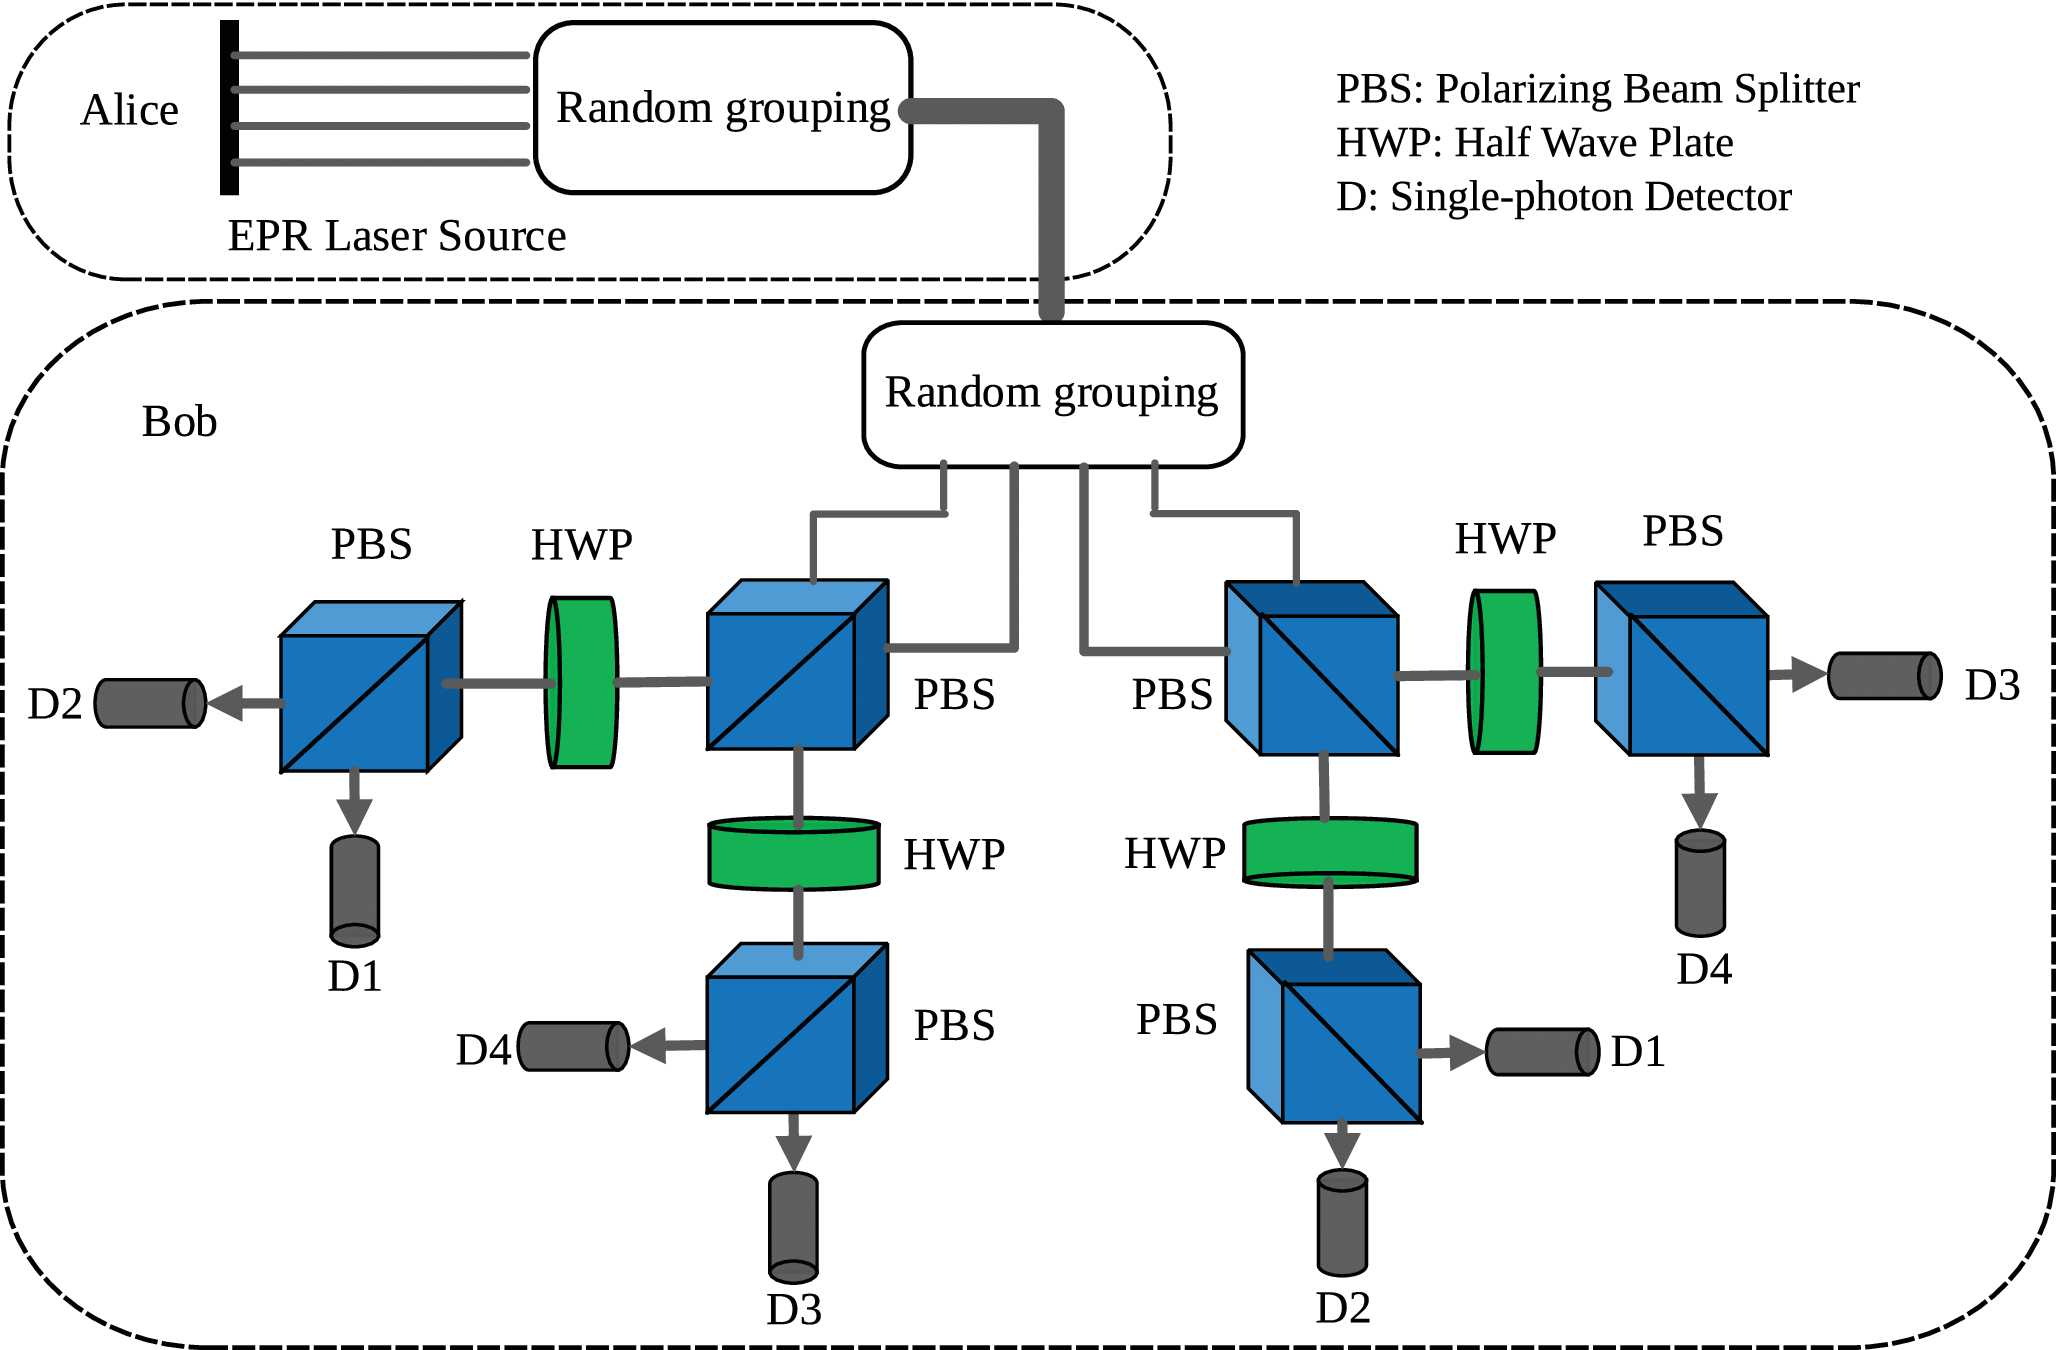
\includegraphics[width=0.7\columnwidth]{scheme.png}
	\caption{Схема работы предлагаемого протокола QKD. Алиса подготавливает состояние из четырех кубитов и отправляет Бобу по квантовому каналу. Затем Боб группирует их случайным образом и измеряет эти кубиты в базисе состояний Белла.}
	\label{im1}
\end{figure}


\subsection{Алгоритм распределения ключей}

\begin{itemize}

\item \textit{Шаг 1. Подготовка состояний.} Алиса подготавливает одну из комбинаций четырёхкубитных состояний, например, представленную в уравнении \eqref{state}. Каждая такая комбинация состоит из четырёх кубитов $P_\gamma$, где $\gamma \in \{1,2,3,4\}$. %Каждой комбинации ставятся в соответствие два информационных бита ключа $\mathcal{K}$.
Алиса запоминает текущее состоянии кубитов. % и соответствующую информацию ключа $\mathcal{K}$.

\item \textit{Шаг 2. Распределение кубитов.} Согласно договорённости Алиса знает, что выбранные четыре кубита сгруппированы как $\{(P_1, P_3), (P_2, P_4)\}$, а Боб -- нет. Алиса случайным образом переставляет эти четыре кубита и отправляет их Бобу по квантовому каналу.

\item \textit{Шаг 3. Измерение состояний Белла.} Боб принимает отправленные ему кубиты и случайным образом разбивает их на две части. После чего он выполняет измерение состояний Белла на этих двух частях и отправляет полученные результаты Алисе по классическому каналу.

\item \textit{Шаг 4. Сравнение результатов.} Алиса принимает результаты Боба и сравнивает их с сохранённой информацией о $P_\gamma$. Если Алиса увидит совпадение, она объявит по классическому каналу $'1'$ и весь процесс коммуникации может перейти к шагу $5$ или вернуться на шаг $1$. Если же совпадения не случится, она объявит $'0'$ и процесс коммуникации начнётся сначала с шага $1$ или оборвётся. 

\item \textit{Шаг 5. Получение согласованных ключей.} После нескольких итераций последовательностей шагов c $1$ по $4$ Алиса и Боб получают двоичную последовательность, которая представляет собой некоторый необработанный ключ $\mathcal{R}$ (сырой). Под $\mathcal{R}_A$ и $\mathcal{R}_B$ будем понимать необработанные ключи Алисы и Боба соответственно. Алиса случайным образом выбирает части $\mathcal{R}_A$ и собирает из них свой согласованный ключ $\mathcal{C}_A$, после чего объявляет позиции выбранных частей по классическому каналу. Затем Боб согласно этим позициям выбирает свой согласованный ключ $\mathcal{C}_B$ из ключа $\mathcal{R}_B$.

\item \textit{Шаг 6. Усиление конфиденциальности.} Из полученного набора битов $\mathcal{C}_B$ Боб выбирает некоторые в качестве битов чётности $\mathcal{D}_B$ и объявляет $\mathcal{D}_B$ вместе с их соответствующими позициями. Аналогичным образом Алиса выбирает свой набор $\mathcal{D}_A$ и сравнивает его с полученным $\mathcal{D}_B$. Если процент битовых ошибок в таком сравнении меньше некоторого наперёд заданного порога, то соединение может считаться безопасным и процесс коммуникации может перейти к следующему шагу $7$; если нет, то необходимо вернуться на шаг $1$ или же окончательно оборвать связь.

\item \textit{Шаг 7. Формирование окончательных ключей.} На последнем шаге окончательно выбираются ключи $\mathcal{R'}_A$ и $\mathcal{R'}_B$, которые будут использоваться для шифрования в дальнейшем процессе коммуникации по классическому каналу. Теоретически, в идеальном случае должно получиться $\mathcal{R'}_A$ = $\mathcal{R'}_B$, где $\mathcal{R'}_A$ --- это необработанный ключ $\mathcal{R}_A$ исключая биты $\mathcal{C}_A$, аналогичное верно для $\mathcal{R'}_B$.
\end{itemize}

\subsection{Анализ доли ошибочных кубитов}

Как уже оговаривалось, существует несколько различных способов группировок кубитов. Без ограничения общности будем считать, что группировка, приведённая в \eqref{state} является правильной, а остальные --- неправильными. Учитывая, что каждая из $m$ группировок получается равновероятно, вероятность правильной группировки для Бобу равна $\frac{1}{m}$. Измеряя состояния Белла, в каждом из случаев Боб может получить любую из перечисленных комбинаций состояний Белла: $\{\ket{\phi^+}, \ket{\phi^-}\}$, $\{\ket{\phi^-}, \ket{\phi^+}\}$, $\{\ket{\psi^+}, \ket{\psi^-}\}$ и $\{\ket{\psi^-}, \ket{\psi^+}\}$.
Отметим, что если Боб выберет правильную группировку, то он может получить правильные состояния Белла с вероятностью $1$. Если в канале нет подслушивающего устройства, то вероятность ошибки $\varepsilon_0$ может быть получена из анализа двоичной случайной последовательности для каждой группировки.

Пусть Боб случайным образом получил неправильную группировку кубитов, например $\{(P_1 , P_2), (P_3 , P_4)\}$. Тогда состояние \eqref{state} можно выразить следующим образом:

\begin{equation}
\ket{\mathcal{C}}_{1234} = \dfrac{1}{2} \Big(\ket{0000} + \ket{0011}
 + \ket{1100} + \ket{1111} \Big)_{1234} = \Big(\ket{\phi^-}_{12} \ket{\phi^+}_{34}\Big).
\end{equation}

В этом случае, при измерении из всех комбинаций состояний Белла он получит только $\ket{\phi^-}_{12} \ket{\phi^+}_{34}$. Сравнивая с \eqref{state}, заключаем, что Боб получит правильную бинарную последовательность $\mathcal{K}$ c вероятностью $\frac{1}{4}$.

Повторяя данные действия для всех возможных группировок, находим, что доля ошибочных кубитов $\varepsilon_0 = 0,0417$ \cite{base}. Взаимная информация Алисы и Боба:

\begin{equation}
\mathcal{I}(A; B) = 1 - [- \varepsilon_0 \log_2 \varepsilon_0 -(1-\varepsilon_0)\log_2(1-\varepsilon_0) ] = 0,7501.
\end{equation}

\section{Криптоанализ}

\subsection{Атака перехвата --- повторной передачи}
Одной из атак на QKD протоколы является атака перехвата --- повторной передачи \cite{ira1, ira2, ira3}. Суть атаки заключается в измерении злоумышленником (Евой) непосредственно квантового состояния носителя (например, фотона) и последующей повторной посылке нового фотона в состоянии, полученном в результате измерения. Поскольку злоумышленник не пропускает квантовые состояния отправителя, а генерирует новые и отправляет их получателю, то данная атака также называется непрозрачной. 

В рассматриваемом случае Ева может взаимодействовать с полученным сообщением и повторно послать Бобу новое состояние из четырех кубитов, чтобы он продолжал получать сообщения. Тогда Ева играет ту же роль, что и Боб в процессе коммуникации. Злоумышленник аналогично Бобу может разбить состояние из четырех кубитов на две части и измерить состояния Белла каждой из них.

После шага $2$ генерации секретного ключа, четыре кубита, отправленные Алисой, будут передаваться по квантовому каналу связи. Предположим, что Ева перехватывает эти четыре кубита и обрабатывает их так же, как и Боб. Затем Ева пересылает свои четыре обновлённых кубита Бобу. 

Перебирая все возможные случаи группировок кубитов Евой и Бобом, можно получить полную вероятность того, что Боб получит неверный результат при измерении состояний Белла. Данная вероятность также называется долей ошибочных кубитов $\varepsilon_e$. Согласно \cite{base} $\varepsilon = 0,1597$.

Найдём число битов двоичной случайной последовательности $n$, которые нужно сравнить Алисе и Бобу, чтобы обнаружить Еву с вероятностью $p_d = 1 - 10^{-9}$:

\begin{equation*}
p_d = 1 - \varepsilon_e ^n.
\end{equation*}
Минимальное значение $n = 11$ (\cite{base}), в то время как Алиса и Боб должны сравнить $n = 72$ в протоколе BB84 (\cite{eleven}), чтобы достичь аналогичной вероятности. 


Из вышеприведенных анализов мы можем вычислить взаимную информацию между Алисой и Евой. 

Вычислим взаимную информацию между Алисой и Евой:  
\begin{equation}
\mathcal{I}(A; E) = 1 - [- \varepsilon_e \log_2 \varepsilon_e -(1-\varepsilon_e)\log_2 (1-\varepsilon_e) ] = 0,3664 \text{ бит}.
\end{equation}

Таким образом, связь безопасна, поскольку $\mathcal{I}(A; B) > \mathcal{I}(A; E)$. Более того, $\mathcal{I}(A; B)$ в рассматриваемом протоколе больше чем $\mathcal{I'} (A; B) = 0,1887$ бит в протоколе BB84.
Теоретическое значение секретности ключа:
\begin{equation}
\mathcal{R} = \mathcal{I}(A; B) - \mathcal{I}(A; E) = 0,7501 - 0,3664 = 0,3837 > 0.
\end{equation}


\subsection{Атака троянского коня}

Атака троянского коня \cite{trojan,trojan2, trojan4}, подразумевает, что система QKD может быть взломана Евой путем отправки яркого света в квантовый канал и анализа обратного отражения. Ева использует вспомогательный источник, модулирует его и анализирует обратно рассеянный сигнал с помощью детектора. Как правило \cite{trojan}, схема обнаружения истинного сигнала основана на особенностях вспомогательного источника, например, на его фазе. Еве необходимо удалить часть истинного сигнала, и затем компенсировать введенные потери с помощью улучшения квантового канала. Следовательно, Еве нужно подготовить канал, который имеет меньшее затухание, чем изначальный квантовый канал. Если это выполнено, Ева может измерить перехваченное состояние с помощью квантовой памяти.

\begin{figure}[h]
	\center{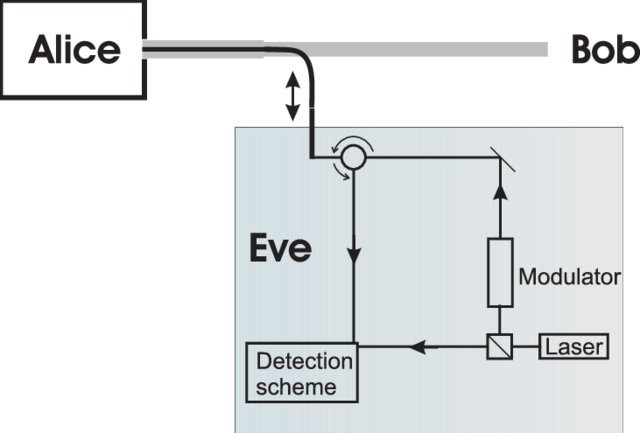
\includegraphics[width=0.5\linewidth]{trojan.jpg}}
	\label{ris:image2}
\end{figure}


При атаке Троянского Коня известно измерение \cite{trojan, trojan3}, которое максимизирует собственную информацию Евы, т.е. информационный выигрыш:

\begin{equation*}
\mathcal{I}_{Eve}(|\alpha|^2) = 1 - h(p),
\end{equation*}

где $p = \frac{1}{2} \big(\sqrt{1 - |\braket{\alpha, 0 | 0, \alpha}|^2 } \big) \approx \frac{1 + \sqrt2 |\alpha|}{2}$, $(p) = -p\log_2(p) - (1-p)\log_2(p)$, $|\alpha|^2$ обозначает номер фотона Евы.

Раскладывая выражение для собственной информации Евы в ряд Тейлора получим:

\begin{align*}
\mathcal{I}_{Eve}(|\alpha|^2) &\approx 1 + 
\Big( \frac{1 + \sqrt2 |\alpha|}{2} \Big) \log_2 \Big(\frac{1 + \sqrt2 |\alpha|}{2}\Big) + \Big( \frac{1 - \sqrt2 |\alpha|}{2} \Big) \log_2 \Big(\frac{1 - \sqrt2 |\alpha]|}{2}\Big) = \nonumber \\
&= 1 - 1 + \frac{(\sqrt2 |\alpha|)^2}{\log4} + \frac{(\sqrt2 |\alpha|)^4}{6\log4} + \mathcal{O}(|\alpha|^6) = \frac{|\alpha|^2}{\log2} + \mathcal{O}(|\alpha|^4).
\end{align*}

Согласно полученному выражению и границам, представленным в \cite{trojan} мы можем заключить \cite{base}, что $\max\limits_{|\alpha|^2} \big\{\mathcal{I}_{Eve} (|\alpha|^2) \big\} < \mathcal{I}(A; B)$. Следовательно, атака троянского коня может
быть предотвращена в рассматриваемом протоколе.

\iffalse ... 
\section{Numerical Appendix}

\begin{equation*}
\ket{\phi^{\pm}} = \dfrac{1}{\sqrt2}\big(\ket{00} \pm \ket{11} \big), \quad
\ket{\psi^{\pm}} = \dfrac{1}{\sqrt2}\big(\ket{01} \pm \ket{10} \big).
\end{equation*}



\begin{align*}
\ket{\mathcal{C}}_{1234} = \ket{\phi^-}_{12} \otimes \ket{\phi^+}_{34}
= \dfrac{1}{2} \big(\ket{00}_{12} - \ket{11}_{12} \big) \otimes \big( \ket{00}_{34} + \ket{11}_{34} \big) = \nonumber \\
= \dfrac{1}{2} \big(\ket{0000} + \ket{0011} - \ket{1100} - \ket{1111}\big)_{1234} =
\end{align*}

\begin{align*}
\ket{\mathcal{C}}_{1234} = \dfrac{1}{2} \Big(\ket{\phi^+}_{13} \ket{\phi^-}_{24} + 
\ket{\phi^-}_{13} \ket{\phi^+}_{24} +
\ket{\psi^+}_{13} \ket{\psi^-}_{24} +
\ket{\psi^-}_{13} \ket{\psi^+}_{24} \Big) = \nonumber \\
\end{align*}

\begin{align*}
\ket{\phi^+}_{m} \ket{\phi^-}_{n} = \dfrac{1}{2} \big(\ket{00}_m \ket{00}_n - \ket{00}_m \ket{11}_n + \ket{11}_m \ket{00}_n - \ket{11}_m \ket{11}_n \big) \nonumber \\
\ket{\phi^-}_{m} \ket{\phi^+}_{n} = \dfrac{1}{2} \big(\ket{00}_m \ket{00}_n + \ket{00}_m \ket{11}_n - \ket{11}_m \ket{00}_n - \ket{11}_m \ket{11}_n \big) \nonumber \\
\ket{\psi^+}_{m} \ket{\psi^-}_{n} = \dfrac{1}{2} \big(\ket{01}_m \ket{01}_n - \ket{01}_m \ket{10}_n + \ket{10}_m \ket{01}_n - \ket{10}_m \ket{10}_n \big)
\nonumber \\
\ket{\psi^-}_{m} \ket{\psi^+}_{n} = \dfrac{1}{2} \big(\ket{01}_m \ket{01}_n + \ket{01}_m \ket{10}_n - \ket{10}_m \ket{01}_n - \ket{10}_m \ket{10}_n \big)
\end{align*}
\fi

\bibliography{ru}

\end{document}

